%%%%%%%%%%%%%%%%%%%%%%%%%%%%%%%%%%%%%%%%%
% Short Sectioned Assignment LaTeX Template Version 1.0 (5/5/12)
% This template has been downloaded from: http://www.LaTeXTemplates.com
% Original author:  Frits Wenneker (http://www.howtotex.com)
% License: CC BY-NC-SA 3.0 (http://creativecommons.org/licenses/by-nc-sa/3.0/)
%%%%%%%%%%%%%%%%%%%%%%%%%%%%%%%%%%%%%%%%%

%----------------------------------------------------------------------------------------
%	PACKAGES AND OTHER DOCUMENT CONFIGURATIONS
%----------------------------------------------------------------------------------------

\documentclass[paper=a4, fontsize=11pt]{scrartcl} % A4 paper and 11pt font size

% ---- Entrada y salida de texto -----

\usepackage[T1]{fontenc} % Use 8-bit encoding that has 256 glyphs
\usepackage[utf8]{inputenc}

% ---- Idioma --------

\usepackage[spanish, es-tabla]{babel} % Selecciona el español para palabras introducidas automáticamente, p.ej. "septiembre" en la fecha y especifica que se use la palabra Tabla en vez de Cuadro

% ---- Otros paquetes ----

\usepackage{amsmath,amsfonts,amsthm} % Math packages
\usepackage{graphics,graphicx, floatrow} %para incluir imágenes y notas en las imágenes
\usepackage{graphics,graphicx, float} %para incluir imágenes y colocarlas
\usepackage{hyperref} % url in references
\usepackage{listings}
\usepackage{color}
\definecolor{grey}{gray}{0.9}

% Para hacer tablas comlejas
\usepackage{multirow}
\usepackage{threeparttable}

\usepackage{fancyhdr} % Custom headers and footers
\pagestyle{fancyplain} % Makes all pages in the document conform to the custom headers and footers
\fancyhead{} % No page header - if you want one, create it in the same way as the footers below
\fancyfoot[L]{} % Empty left footer
\fancyfoot[C]{} % Empty center footer
\fancyfoot[R]{\thepage} % Page numbering for right footer
\renewcommand{\headrulewidth}{0pt} % Remove header underlines
\renewcommand{\footrulewidth}{0pt} % Remove footer underlines
\setlength{\headheight}{13.6pt} % Customize the height of the header

\numberwithin{equation}{section} % Number equations within sections (i.e. 1.1, 1.2, 2.1, 2.2 instead of 1, 2, 3, 4)
\numberwithin{figure}{section} % Number figures within sections (i.e. 1.1, 1.2, 2.1, 2.2 instead of 1, 2, 3, 4)
\numberwithin{table}{section} % Number tables within sections (i.e. 1.1, 1.2, 2.1, 2.2 instead of 1, 2, 3, 4)

\setlength\parindent{0pt} % Removes all indentation from paragraphs - comment this line for an assignment with lots of text

\newcommand{\horrule}[1]{\rule{\linewidth}{#1}} % Create horizontal rule command with 1 argument of height

\usepackage{textcomp}
\usepackage{hyperref}

%----------------------------------------------------------------------------------------
%	DATOS
%----------------------------------------------------------------------------------------

\newcommand{\myName}{Francisco Javier Bolívar Lupiáñez}
\newcommand{\myColleageName}{Juan Pablo González Casado}
\newcommand{\myDegree}{Máster en Ingeniería Informática}
\newcommand{\myFaculty}{E. T. S. de Ingenierías Informática y de Telecomunicación}
\newcommand{\myDepartment}{Ciencias de la Computación e Inteligencia Artificial}
\newcommand{\myUniversity}{\protect{Universidad de Granada}}
\newcommand{\myLocation}{Granada}
\newcommand{\myTime}{\today}
\newcommand{\myTitle}{Práctica 2}
\newcommand{\mySubtitle}{Clasificación de Imágenes}
\newcommand{\mySubject}{Sistemas Inteligentes para la Gestión de la Empresa}
\newcommand{\myYear}{2016-2017}

%----------------------------------------------------------------------------------------
%	PORTADA
%----------------------------------------------------------------------------------------


\title{	
	\normalfont \normalsize 
	\textsc{\textbf{\mySubject \space (\myYear)} \\ \myDepartment} \\[20pt] % Your university, school and/or department name(s)
	\textsc{\myDegree \\[10pt] \myFaculty \\ \myUniversity} \\[25pt]
	\horrule{0.5pt} \\[0.4cm] % Thin top horizontal rule
	\huge \myTitle: \mySubtitle \\ % The assignment title
	\horrule{2pt} \\[0.5cm] % Thick bottom horizontal rule
	\normalfont \normalsize
}

\author{
	\myName \\ 
	\myColleageName \\ \\ 
	\small Kaggle: \texttt{EchaEquipos} \\
	\small Posición: 195, Puntuación: 0.80378 \\ 
}

\date{\myTime} % Incluye la fecha actual
%----------------------------------------------------------------------------------------
%	INDICE
%----------------------------------------------------------------------------------------

\begin{document}
	
\definecolor{light-gray}{gray}{0.95}
	
\lstset {
	basicstyle=\scriptsize,
	frame=single,
	backgroundcolor=\color{grey}
}

\lstdefinestyle{R}{
	frame=single,
	numbers=left,
	language=R,
	basicstyle=\tiny\ttfamily,
	keywordstyle=\bfseries,
	commentstyle=\itshape,
	identifierstyle=\bfseries,
}
	
\setcounter{page}{0}

\maketitle % Muestra el Título
\thispagestyle{empty}

\newpage %inserta un salto de página

\tableofcontents % para generar el índice de contenidos

%\listoftables
%\listoffigures

\newpage

%----------------------------------------------------------------------------------------
%	DOCUMENTO
%----------------------------------------------------------------------------------------

\section{Exploración de datos}

Los datos que tenemos son una serie de imágenes a color con un tamaño de 3096 x 4128 y un peso aproximado que ronda de entre 2.5 a 7.5 MB.
\\ \\
Estas imágenes son fotos de cérvix femenina (parte inferior del útero) echadas desde distintas distancias y ángulos.
\\ \\
En el caso de las imágenes de \textit{train} las tenemos estructuradas en tres directorios distintos (\texttt{Type\_1}, \texttt{Type\_2} y \texttt{Type\_3}), uno por cada clase. En el caso de las imágenes de \textit{test} las tenemos todas en un solo directorio pues desconocemos el tipo de cada uno y es que ese será el objetivo de la práctica: clasificar cada una de estas 512 imágenes en los tres tipos distintos.
\\ \\
El conjunto de datos de \textit{train} consta 1481 imágenes, no obstante Kaggle proporciona más imágenes adicionales para aumenta a 7004 el número de imágenes para entrenar nuestros modelos.

\subsection{Dataset no balanceado}

Lo primero que podemos observar es que tanto el conjunto básico (Figura \ref{fig:num-images-train-dataset}) como el que incluye las imágenes adicionales (Figura \ref{fig:num-images-train-extra-dataset}) se encuentran desequilibrados con pocas imágenes del tipo 1 y muchas de los tipos 2 y 3. Esto es algo que tendremos que tener muy en cuenta a la hora de realizar el preprocesamiento de datos.

\begin{figure}[H]
	\centering
	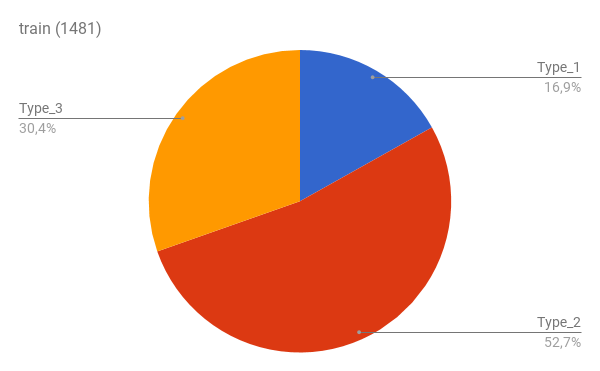
\includegraphics[width=12cm]{img/num-images-train-dataset}
	\caption{Porcentaje de imágenes de cada tipo para el \textit{dataset} básico}
	\label{fig:num-images-train-dataset}
\end{figure}

\begin{figure}[H]
\centering
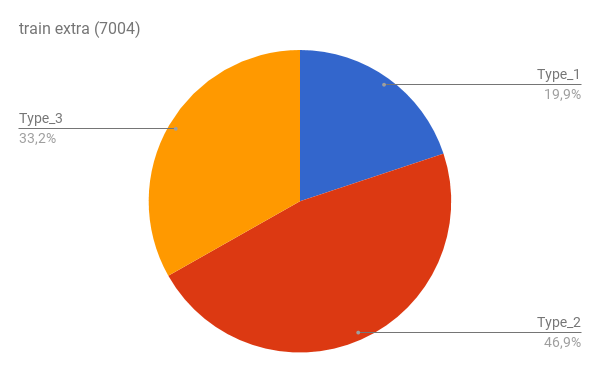
\includegraphics[width=12cm]{img/num-images-train-extra-dataset}
\caption{Porcentaje de imágenes de cada tipo para el \textit{dataset} que incluye las imágenes adicionales}
\label{fig:num-images-train-extra-dataset}
\end{figure}

\subsection{Imágenes que no corresponden a un cérvix}

Además, a la hora de explorar cada uno de estos datos, nos encontramos con imágenes que no correspondían a un cérvix o se encontraban demasiado borrosas (Figura \ref{fig:no-cervix-image}). En Kaggle hay un foro de discusión sobre esto \cite{ImagesExcluded}. Obviamente, en el posterior proceso de preprocesamiento de datos se eliminarán para que no agreguen ningún tipo de ruido a nuestro modelo.

\begin{figure}[H]
	\centering
	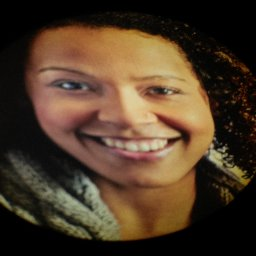
\includegraphics[width=3.5cm]{img/3086}
	
\includegraphics[width=3.5cm]{img/4065}
	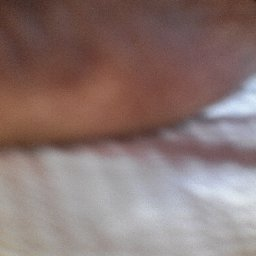
\includegraphics[width=3.5cm]{img/4533}
	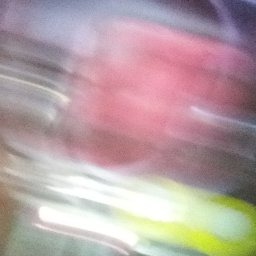
\includegraphics[width=3.5cm]{img/4367}
	\caption{Ejemplos de imágenes que se encuentran en el \textit{dataset} pero no corresponden a un cérvix o se encuentran demasiado borrosas}
	\label{fig:no-cervix-image}
\end{figure}

\section{Preprocesamiento de datos}

Como comenté en la sección anterior. Lo primero que hicimos fue borrar todas las fotos que no correspondían a cérvix o estaban demasiado borrosas. Después de esto nos planteamos realizar \textit{data augmentation}. Para ello realizamos varios \textit{scripts} en R con los que realizábamos operaciones de rotación y volteo para generar hasta ocho imágenes más por cada imagen. No obstante no llegamos a utilizarlos por problemas en memoria en nuestros equipos, y es que ni siquiera podíamos leer a un tamaño de 224 x 224 (necesario para \textit{fine-tuning}) las 7000 imágenes de Kaggle.
\\ \\
Como hacía falta reducir el número de imágenes se aprovechó para hacer \textit{undersampling} y balancear el conjunto de datos (Figura \ref{fig:num-images-train-extra-balanced-dataset}). No se equilibró totalmente pero se hizo lo suficiente como para que dejase de ser un conjunto de datos desequilibrado.

\begin{figure}[H]
	\centering
	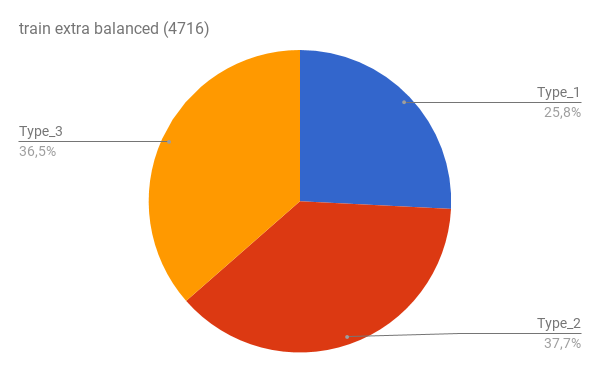
\includegraphics[width=12cm]{img/num-images-train-extra-balanced-dataset}
	\caption{Porcentaje de imágenes de cada tipo para el \textit{dataset} que incluye las imágenes adicionales al que posteriormente se le ha realizado \textit{undersampling} para balancearlo.}
	\label{fig:num-images-train-extra-balanced-dataset}
\end{figure}

El conjunto de datos final cuenta con 4716 imágenes (1217 del primer tipo, 1780 del segundo y 1719 del tercero).

\section{Técnicas de clasificación}

\subsection{\textit{Learning from scratch}}

Lo primero que hicimos fue crear una CNN (\textit{Convolutional Neural Network}) desde cero. Para ello intentamos realizarlo con MXNet en R. Pero tras varios días lanzando el \textit{script} con distintos parámetros no conseguíamos que predijese porcentajes distintos para cada imagen. Y es que al principio pensábamos que era por culpa de la red simple que usábamos pero al probar con una topología famosa (AlexNet) y seguir obteniendo estos resultados, empezamos a sospechar que era algún error de programación en el \textit{script}. Lo depuramos para intentar encontrar el \textit{bug}, pero al no encontrarlo pasamos a utilizar Keras en Python.
\\ \\
Comenzamos siguiendo un \textit{kernel} \cite{StartKernel} con el que se garantizaba bajar el \textit{loss} de 1.
\\ \\
Este \textit{kernel} redimensiona y normaliza las imágenes, realiza \textit{data augmentation}, genera un conjunto de validación a partir de los datos de \textit{train} y entrena una red neuronal simple (Figura \ref{fig:kernel-cnn}) con la que posteriormente predice y exporta a CSV.

\begin{figure}[H]
	\centering
	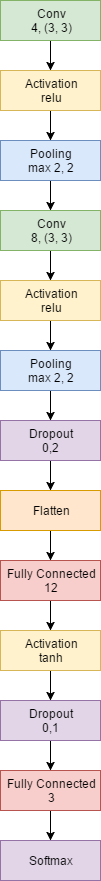
\includegraphics[height=17cm]{img/kernel-cnn}
	\caption{Topología de la red usada en el \textit{kernel} básico que se ha utilizado como base.}
	\label{fig:kernel-cnn}
\end{figure}

Se empezó utilizando el conjunto de datos de \textit{train} completo (pues todavía no se había realizado el \textit{undersampling} para el balanceo).
\\ \\
Se probó a variar el número de épocas para ver cuándo se estancaba la pérdida de \textit{loss} (o subía) en el conjunto de validación para detectar cuando sobre aprendía.
\\ \\
También se probó a variar el tamaño de las imágenes y vimos como con una red tan simple apenas se notaba la diferencia y se podían usar imágenes de incluso 32x32 obteniendo resultados similares a los obtenidos con imágenes de 128x128.
\\ \\
Lo siguiente que se probó a variar fue el tamaño del \textit{batch} y el \textit{samples per epoch}. Viendo que si se aumentaba este segundo parámetro se llegaba a aprender en menor número de épocas.
\\ \\
Por último se probó a hacer más compleja la red neuronal agregando dos ciclos más de capas \textit{Convolution}, \textit{Activation}, \textit{Pooling}, así como agregar más capas \textit{Fully Connected}. Sin embargo lo único que se consiguió con esto fue aumentar el tiempo de cómputo, que era casi despreciable con el modelo sencillo, porque los resultados eran ligeramente peores que los obtenidos anteriormente con la CNN simple.
\\ \\
¿A qué se debe esto? Quizás a que no se dejó entrenar durante un buen número de épocas. Pero sobre todo a que estábamos creando una topología a ciegas. Para perder horas de cómputo con esta red compleja, ¿por qué no probar con una topología que ha dado buenos resultados en otros problemas?
\\ \\
Era hora de pasar a probar el \textit{fine-tuning}.

\subsection{\textit{Fine-tuning}}

Con el \textit{fine-tuning} nos encontramos muchísimos problemas. No en la implementación que se encuentra publicada en la propia web de Keras \cite{KerasApplications}.
\\ \\
Estos problemas eran relacionados con las limitaciones \textit{hardware} de nuestros equipos.
\\ \\
El primero de ellos nos impedía entrenar la CNN y es que no teníamos memoria suficiente para alojar a un tamaño de 224x224 (necesario para la mayoría de las redes) las 7000 fotos que proporciona Kaggle. Es entonces cuando aprovechamos para hacer el \textit{undersampling} y consecuente balanceo del \textit{dataset}.
\\ \\
El segundo problema era el del tiempo de cómputo. Pues al no contar con GPU una sola época duraba entre 40 y 80 minutos dependiendo de la topología. Lo que nos impedía realizar experimentos con agilidad. Por ello nos llevó varios días dejando entrenar la CNN hasta 13 horas. Por suerte, los dos últimos días se pudo contar con una GPU que reducía enormemente estos tiempos pasando de 40 minutos a 40 segundos por época. Pero era demasiado tarde y apenas se pudieron realizar unos pocos experimentos.
\\ \\
Se probó como base las topologías \textit{VGG16}, \textit{VGG19} y \textit{ResNet50} llegando a hacer \textit{submissions} solo con esta última pues no se consiguió que se aprendiese con las dos primeras. El \textit{log loss} era muy alto tras varias épocas incluso para el conjunto de datos de \textit{train}.
\\ \\
Se crearon tres topologías utilizando \textit{ResNet50} (Figura \ref{fig:fine-tuning-topologies}):

\begin{itemize}
	\item Una primera en la que se conectaba directamente la salida de ResNet50 a una capa \textit{Flatten}, una \textit{Fully Connected} de tamaño 3 (las tres posibles salidas) que se conecta con una activación \textit{softmax}.
	\item Otra utilizando la misma que se muestra en la web de Keras \cite{KerasApplications}.
	\item Otra igual a la anterior pero disminuyendo los nodos de la capa \textit{Fully Connected}.
\end{itemize}

\begin{figure}[H]
	\centering
	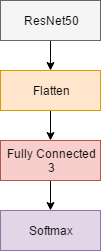
\includegraphics[width=2cm]{img/fine-tuning-topology-1}
	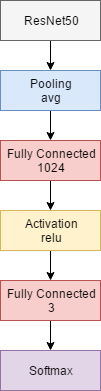
\includegraphics[width=2cm]{img/fine-tuning-topology-2}
	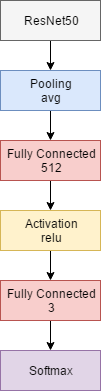
\includegraphics[width=2cm]{img/fine-tuning-topology-3}
	\caption{Topologías utilizadas para el \textit{fine-tuning}.}
	\label{fig:fine-tuning-topologies}
\end{figure}

Con la primera topología no se consiguieron buenos resultados y con la segunda se veía como sobreaprendía muy rápidamente. Fue con la última de ellas con la que se consiguió mejorar los resultados obtenidos usando \textit{learning from scratch}.
\\ \\
Al igual que se hizo con \textit{learning from scratch} se probó a cambiar distintos parámetros hasta obtener mejores resultados.
\\ \\
Además se probó a realizar el entrenamiento solo sobre las capas añadidas manualmente tras \textit{ResNet50}, entrenando también algunas de la red importada o realizando un entrenamiento en dos fases. La primera (durante pocas épocas) con un ratio de aprendizaje mayor sobre las capas añadidas manualmente y la segunda con un ratio de aprendizaje menor también sobre las últimas capas de \textit{ResNet50}.
\\ \\
Se observó como el \textit{log loss} sobre el conjunto de \textit{train} disminuía continuamente hasta la época que se dejó mientras que el de validación se estancaba antes en 0,8. Con el conjunto de \textit{test}, al subir los resultados a Kaggle, se vio que empezaba a dar peores resultados antes (Figura \ref{fig:loss-variation-fine-tuning}).

\begin{figure}[H]
	\centering
	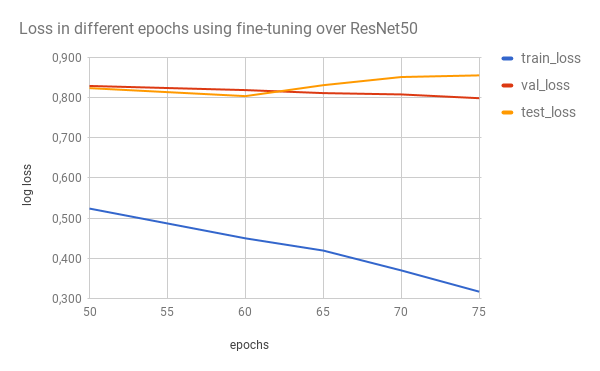
\includegraphics[width=12cm]{img/loss-variation-fine-tuning}
	\caption{Variación de \textit{log loss} en los distintos conjuntos de datos a lo largo de las épocas.}
	\label{fig:loss-variation-fine-tuning}
\end{figure}

En el gráfico (Figura \ref{fig:loss-variation-fine-tuning}) se muestrea en las épocas 50, 60, 65, 70 y 75. Obteniendo el mejor resultados en la 60. Sin embargo, no sabemos con certeza si entre la época 50 y 60 o la 60 y 65 hay un resultado mejor. Y es que elegir en qué época exacta parar de entrenar es complicado, aunque elegir una aproximada si puede resultar más sencillo viendo cómo se comporta el \textit{log loss} en los conjuntos de \textit{train} y validación pues nos pueden estar dando pistas de cuándo está sobreaprendiendo. En el caso de ejemplo que mostramos se ve cómo a partir de la época 65 aumenta el ritmo de bajada en el conjunto de \textit{train} y no en el de validación. A partir de la época 75 (no aparece en la gráfica) el \textit{log loss} sobre el conjunto de validación se estancaba llegando a aumentar en las épocas posteriores. Estos dos hechos nos hacen despreciar lo que pase a partir de estas épocas y centrarnos en las anteriores para buscar el mejor resultado posible.

\subsection{\textit{OVO} y \textit{OVA}}

Hasta ahora se ha realizado clasificación multiclase en la que la red neuronal tenía una salida \textit{softmax} con tres nodos, uno correspondiente a cada clase.
\\ \\
El siguiente enfoque es probar otras dos técnicas distintas a la hora de clasificar utilizando las mismas CNN. Estas dos técnicas tratan de convertir el problema de clasificación multiclase en problemas de clasificación binarios y son One vs. One (OVO) y One vs. All (OVA), también conocido como One vs. Rest (OVR).

\subsubsection{\textit{OVO}}

Usando OVO se entrenarán tres clasificadores distintos para distinguir entre dos clases: Tipo 1 vs. Tipo 2, Tipo 1 vs. Tipo 3 y Tipo 2 vs. Tipo 3.
\\ \\
Obviamente, para cada clasificador se utilizarán como entrenamiento las imágenes de los tipos que se comparan, ignorando la del tipo que no está comparando.
\\ \\
Una vez entrenados se va a predecir el tipo de cada imagen pasándola por cada clasificador que obtendrá como salida dos porcentajes, uno por cada uno de los dos tipos. Estos porcentajes se combinarán para obtener el resultado final de porcentaje para cada uno de los tres tipos.
\\ \\
Para combinar estos datos no hay ningún método preestablecido y se podrían utilizar varias técnicas. Por ejemplo, supongamos que tenemos estas salidas:

\begin{itemize}
	\item Tipo 1: 0,7 vs Tipo 2: 0,3
	\item Tipo 1: 0,55 vs Tipo 3: 0,45
	\item Tipo 2: 0,4 vs Tipo 3: 0,6
\end{itemize}

Se podría multiplicar las dos salidas de cada tipo y normalizarlas para que la suma de los tres porcentajes sea 1.

\begin{itemize}
	\item Combinación tipo 1: $ 0,7 \times 0,55 = 0,385 $
	\item Combinación tipo 2: $ 0,3 \times 0,4 = 0,12 $
	\item Combinación tipo 3: $ 0,45 \times 0,6 = 0,27 $
	\item Tipo 1 + Tipo 2 + Tipo 3 = $ 0,385 + 0,12 + 0,27 = 0,775 $
	\item Salida tipo 1: $ \frac{0,385}{0,775} = 0.5 $
	\item Salida tipo 2: $ \frac{0,12}{0,775} = 0.15 $
	\item Salida tipo 3: $ \frac{0,27}{0,775} = 0.35 $
\end{itemize}

Otra opción podría ser realizar la media que directamente obtiene una salida normalizada:

\begin{itemize}
	\item Salida tipo 1: $ \frac{0,7 + 0,55}{3} = 0.42 $
	\item Salida tipo 2: $ \frac{0,3 + 0,4}{3} = 0.23 $
	\item Salida tipo 3: $ \frac{0,45 + 0,6}{3} = 0.35 $
\end{itemize}

\subsubsection{\textit{OVA}}

Usando OVA se utilizarán también otros tres clasificadores pero esta vez distinguirán entre una clase y el resto: Tipo 1 vs. Tipo 2-3, Tipo 2 vs. Tipo 1-3 y Tipo 3 vs. Tipo 1-2.
\\ \\
Para ello se pueden crear tres directorios nuevos combinando las imágenes de dos de los tipos y crear los clasificadores igual que con OVO. 
\\ \\
Para combinar los resultados tampoco hay ningún método estipulado. El método más sencillo que se nos ha ocurrido es utilizar las salidas en las que el tipo hace de \textit{one} y normalizarlas para que sus sumas sean 1.
\\ \\
Por ejemplo, supongamos que tenemos estas salidas en los distintos clasificadores:

\begin{itemize}
	\item Tipo 1: 0,55 vs Tipo 2-3: 0,45
	\item Tipo 2: 0,4 vs Tipo 1-3: 0,6
	\item Tipo 3: 0,1 vs Tipo 1-2: 0,9
\end{itemize}

La salida final sería:

\begin{itemize}
	\item Salida tipo 1: $ \frac{0,55}{0,55 + 0,4 + 0,1} = 0.52 $
	\item Salida tipo 2: $ \frac{0,4}{0,55 + 0,4 + 0,1} = 0.38 $
	\item Salida tipo 3: $ \frac{0,1}{0,55 + 0,4 + 0,1} = 0.1 $
\end{itemize}

\subsection{Extracción de características}

Hasta ahora, ya sea en \textit{learning from scratch} o \textit{fine-tuning}, o en clasificación multiclase, OVO u OVA, la técnica utilizada para predecir ha sido una CNN. No obstante hay más posibilidades para predecir clases.
\\ \\
Una de ellas es la extracción de características extrayendo los mapas de características de la CNN para su posterior uso en técnicas clásicas de \textit{machine learning} como \textit{random forest}, \textit{boosting} o SVM (\textit{Support Vector Machine}).
\\ \\
Para la extraer las características de una CNN usando Keras se puede seguir el ejemplo que hay en su documentación \cite{KerasApplications}. Y es que se haría igual que como se ha venido haciendo hasta ahora pero definiendo como salida del modelo a la hora de predecir la capa donde se encuentran los mapas de características.
\\ \\
Una vez obtenemos los mapas de características podemos usar la librería \textit{scikit-learn} \cite{Sklearn} donde encontramos distintas técnicas como el \textit{random forest} y el SVM \cite{KerasAndSklearn}.

\subsection{\textit{Ensemblers}}

Por último, se podría realizar un \textit{ensembler} con el que combinar varias de las técnicas citadas anteriormente con el objetivo de obtener un mejor resultado.

\section{Presentación y discusión de resultados}

Lala

\section{Conclusiones y trabajo futuro}

Lala

\section{Listado de soluciones}

Lala

%----------------------------------------------------------------------------------------
%	REFERENCIAS
%----------------------------------------------------------------------------------------

\newpage

\bibliography{referencias} %archivo referencias.bib que contiene las entradas 
\bibliographystyle{plain} % hay varias formas de citar

\end{document}